\documentclass[french]{beamer}

\usepackage[utf8]{inputenc}
\usepackage[T1]{fontenc}
\usepackage{verbatim}

\usetheme{Warsaw}


\begin{document}

	\begin{frame}
	\begin{center}
	Topic C : seeing the arrow of time
\newline
\newline
Alban Pierre

11th January 2016
\end{center}
	\end{frame}
	
	\begin{frame}
	
  \tableofcontents[]
\end{frame} 

	\section{Introduction}
	\begin{frame}
	\frametitle{Introduction}
	
	Humans can see if a video is running forward or backward.
	\newline
	\begin{figure}[h]
		\begin{minipage}[b]{.30\linewidth}
			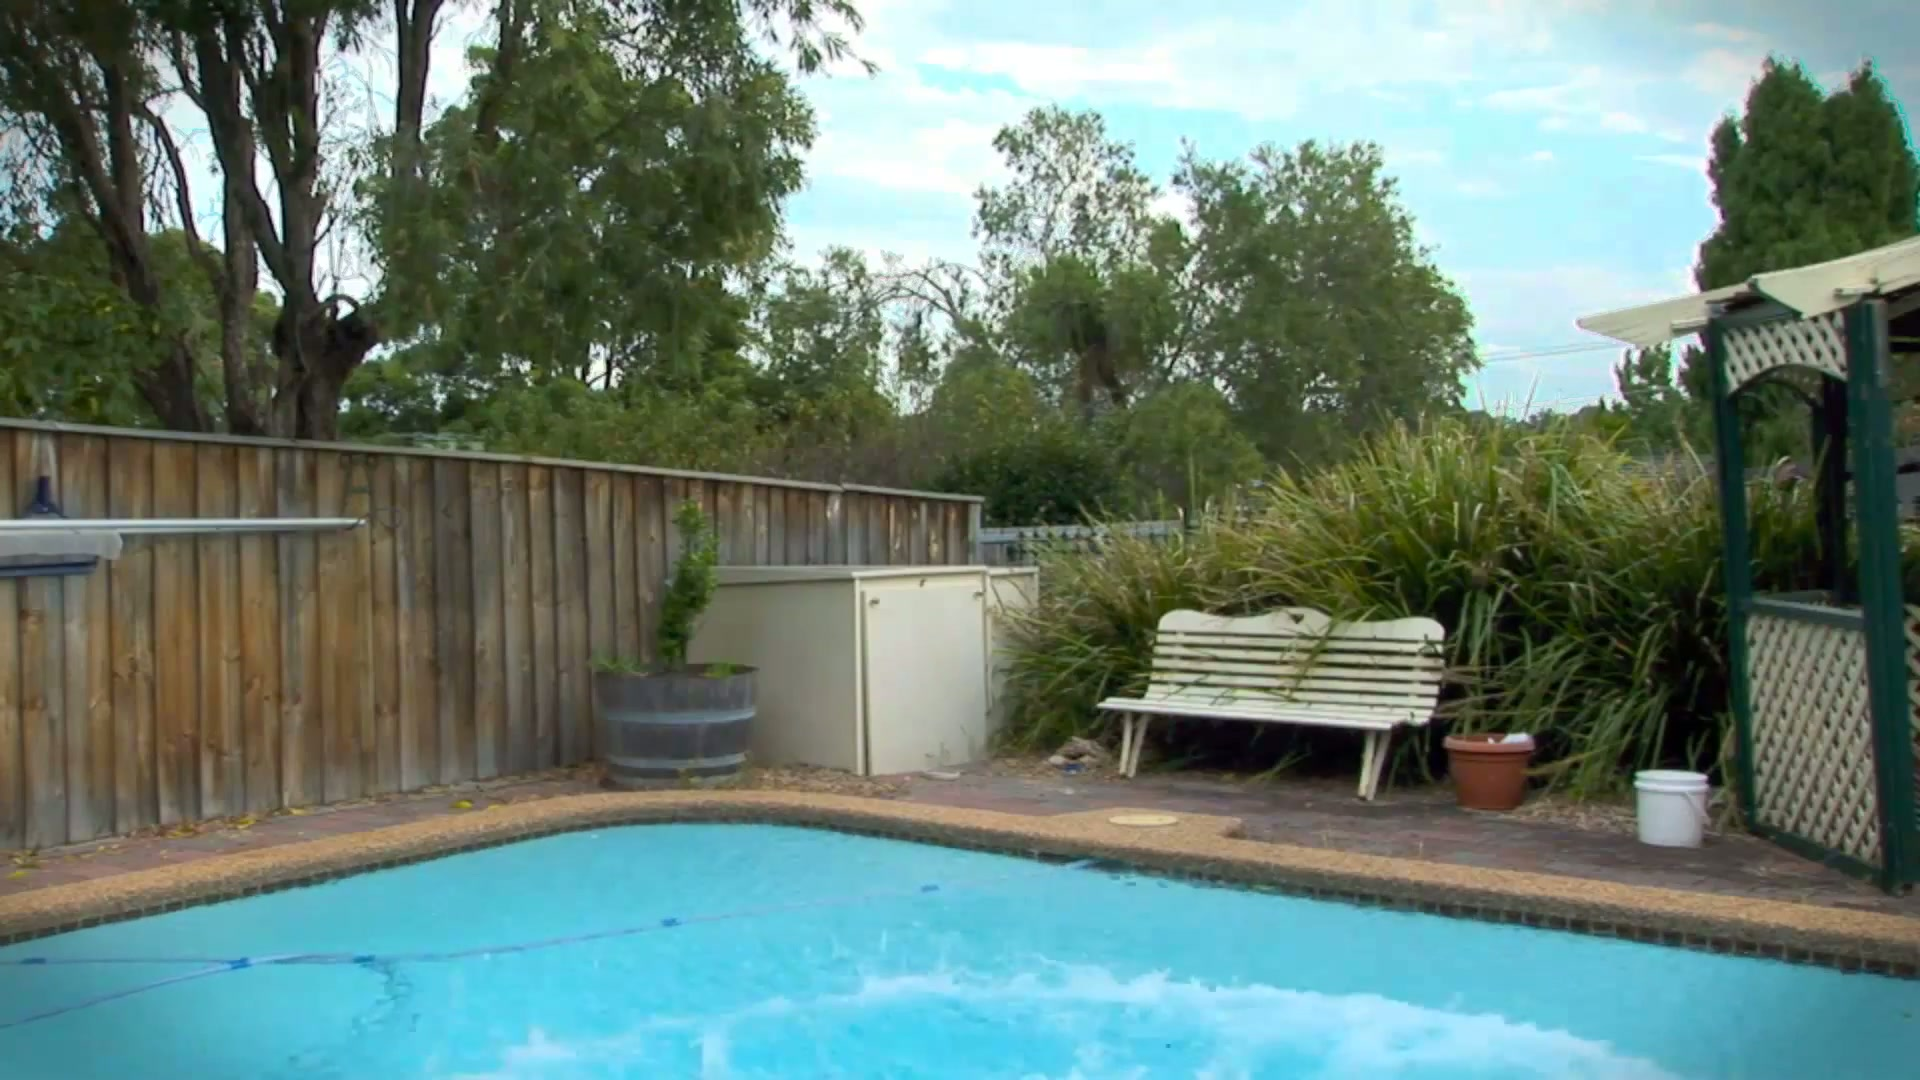
\includegraphics[width=1.0\textwidth]{im01.jpeg}
			%\caption{1000 first iterations (3*2, one)}
		\end{minipage}
		\hspace{5pt}
		\begin{minipage}[b]{0.30\linewidth}
			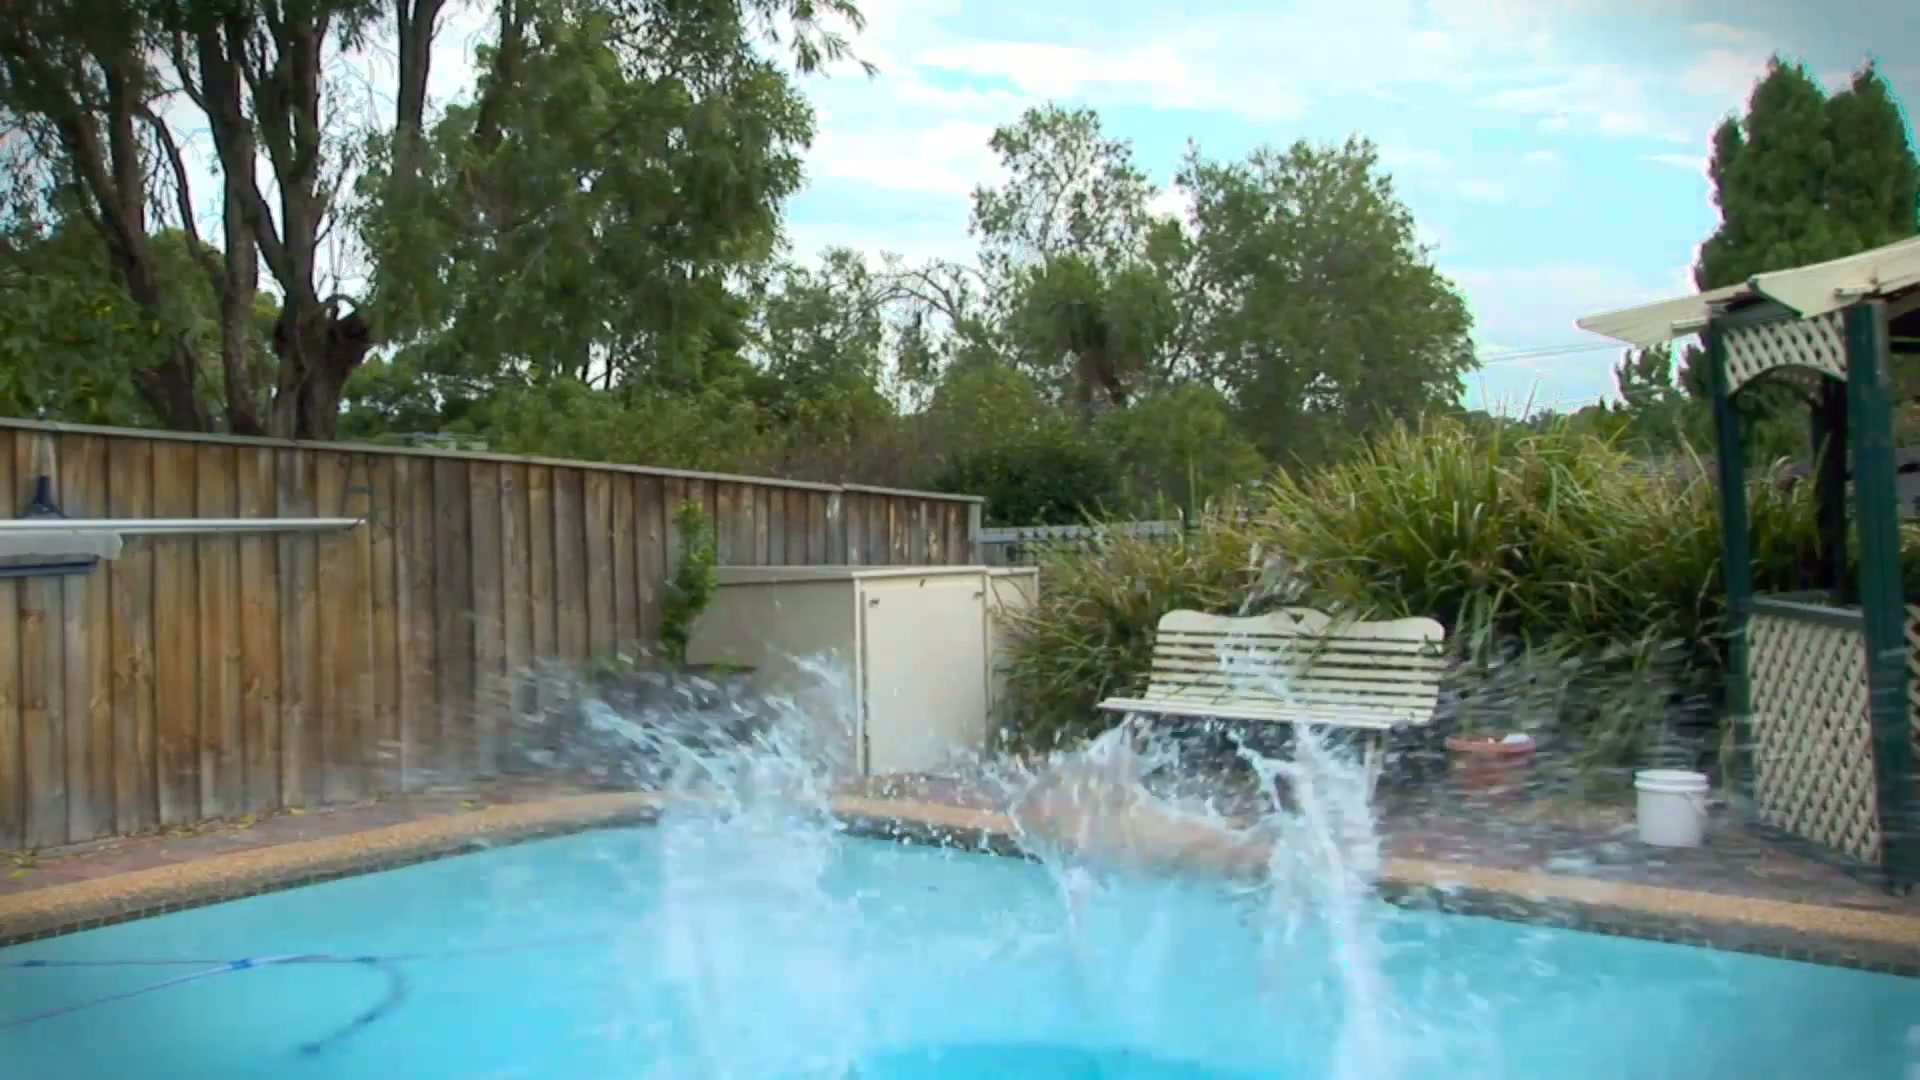
\includegraphics[width=1.0\textwidth]{im30.jpeg}
			%\caption{1000 last iterations (3*2, one)}
		\end{minipage}
		\hspace{5pt}
		\begin{minipage}[b]{0.30\linewidth}
			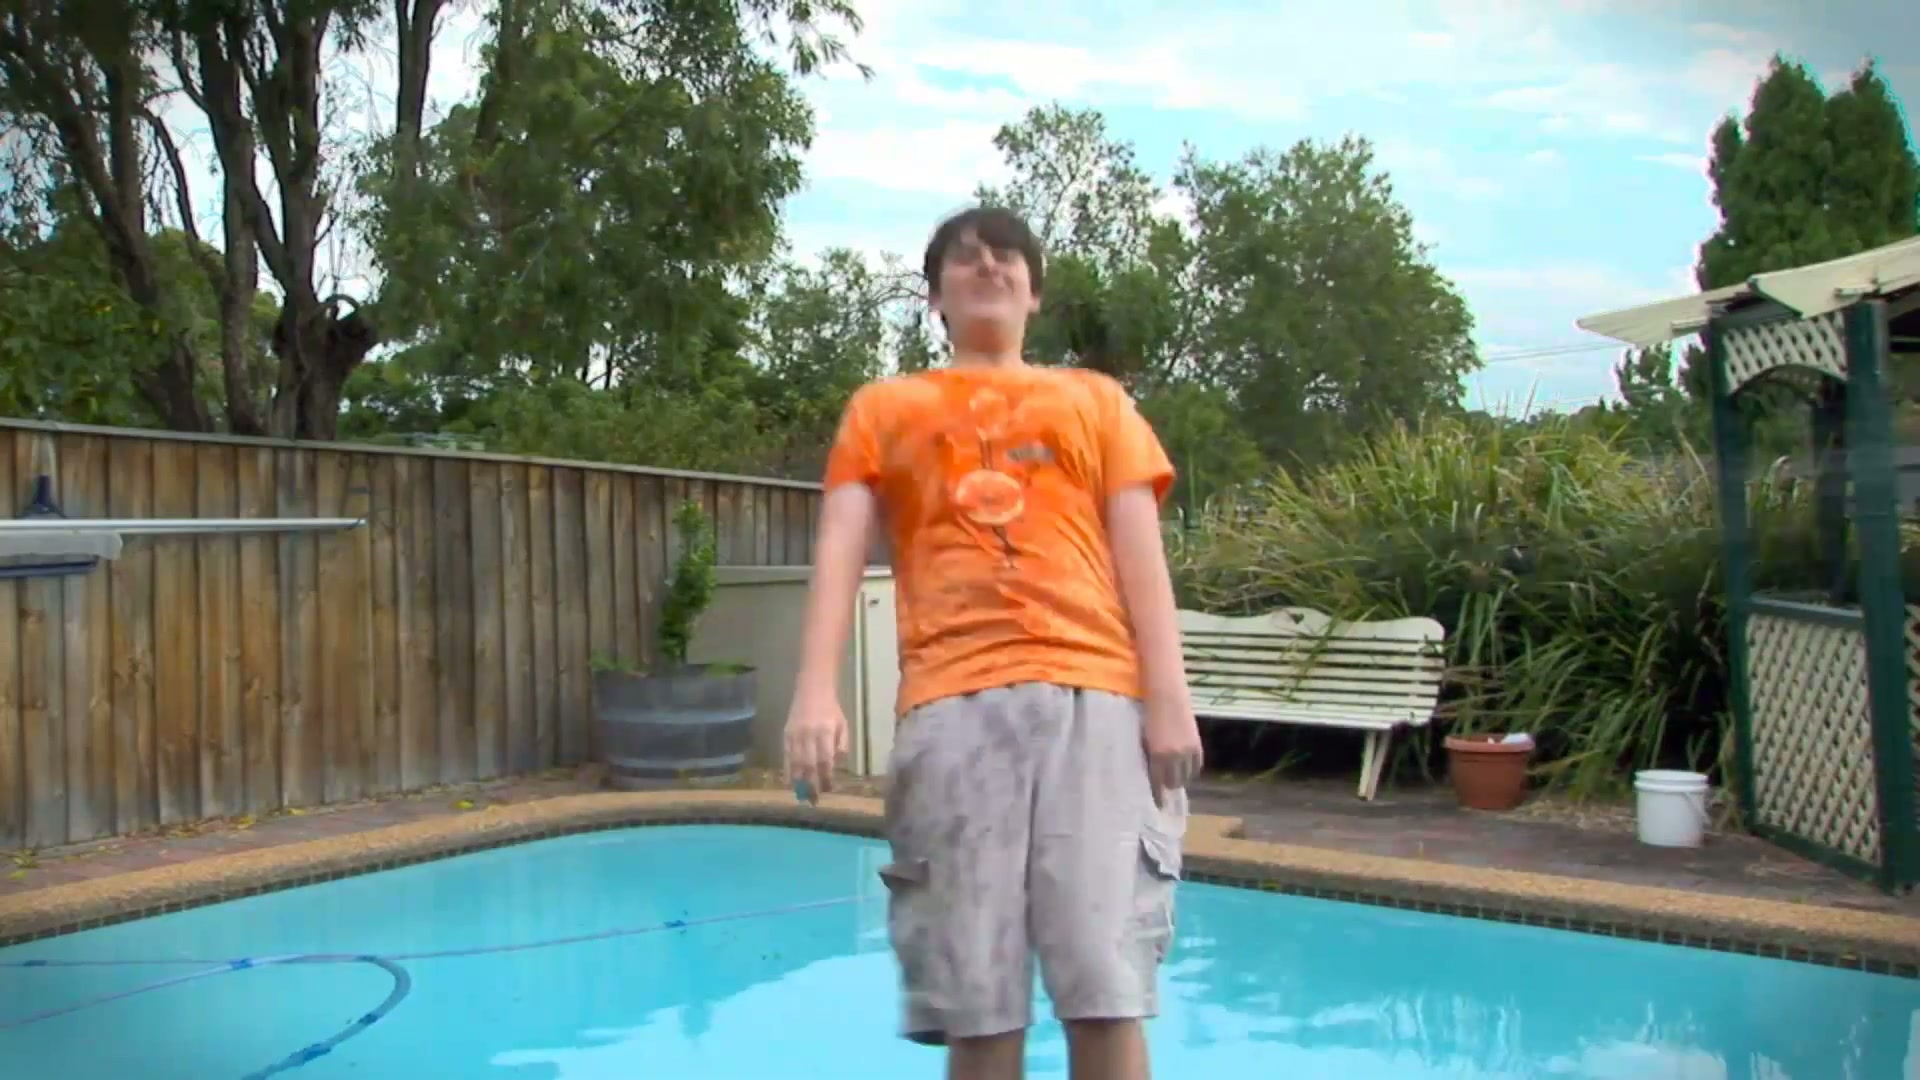
\includegraphics[width=1.0\textwidth]{im50.jpeg}
			%\caption{1000 last iterations (3*2, one)}
		\end{minipage}
		\label{fig:f}
	\end{figure}
	
	$\rightarrow$ Can an algorithm do the same ?
	
	\end{frame}
	
	\begin{frame}
	\section{General structure}
	\frametitle{General structure}
	
	\begin{itemize}
		\item Compute motion descriptors
		\item Take only the meaningful descriptors
		\item Run k-means
		\item Construct histograms
		\item Run SVM classifier (barrier method)
	\end{itemize}
	\end{frame}
	
	
	\begin{frame}
		\section {Computation of descriptors}
		\frametitle{Optical flow descriptors}
		
		\begin{itemize}
			\item Assumes brightness constancy $f(x,y,t) = f(x+dx, y+dy, t+dt)$
			\item Assumes small motions $f(x+dx,y+dy,t+dt) = f(x,y,z) + \frac{\partial f}{\partial x}dx + \frac{\partial f}{\partial y}dy + \frac{\partial f}{\partial t}dt$
		\end{itemize}
		
		\[u = u_{av} - fx\frac{fx u_{av} + fy v_{av} + ft}{\alpha + fx^2 + fy^2}\]
		\[v = v_{av} - fy\frac{fx u_{av} + fy v_{av} + ft}{\alpha + fx^2 + fy^2}\]
	\end{frame}
	
	
	\begin{frame}
		\frametitle{}
		
	\end{frame}
	
	
	\begin{frame}
		\frametitle{}
		
	\end{frame}
	
	
	\begin{frame}
		\frametitle{}
		
	\end{frame}
	
	\begin{frame}
	\frametitle{Remerciements}
	
	Thank you for your attention !
	
	\end{frame}

\end{document}






